\documentclass[compress,12pt]{beamer}

\usetheme{Arguelles}

\usepackage{graphicx}
\usepackage{caption}
\usepackage[spanish,es-noshorthands]{babel}
\usepackage[pages=some]{background}

\usepackage{tikz}
\usepackage{tikz-cd}
\usetikzlibrary{
  babel,
  arrows.meta,
  calc,
  positioning,
  overlay-beamer-styles,
  shadows.blur
}
\usetikzlibrary{decorations.pathmorphing}

\usepackage{amsmath,amssymb,latexsym,amscd} 
\usepackage[all,cmtip]{xy}
\usepackage{fancyhdr}
\usepackage{mathalfa}
\usepackage{mathrsfs}
\usepackage{hyperref}
\usepackage{ragged2e}
\usepackage{wasysym}
\usepackage[numbers]{natbib}

% Colores para la diapositiva Top/Frm
\definecolor{TopBlue}{RGB}{14,73,160}
\definecolor{FrmGreen}{RGB}{15,120,45}
\definecolor{TopLight}{RGB}{235,242,252}
\definecolor{FrmLight}{RGB}{235,248,238}

\pagenumbering{arabic}

\DeclareMathOperator{\op}{op}
\DeclareMathOperator{\pt}{pt}
\DeclareMathOperator{\tp}{tp}
\DeclareMathOperator{\Sp}{sp}
\DeclareMathOperator{\SP}{Sp}
\DeclareMathOperator{\Sob}{Sob}
\DeclareMathOperator{\spec}{spec}
\DeclareMathOperator{\Fit}{Fit}
\DeclareMathOperator{\Fil}{Fil}
\DeclareMathOperator{\Pth}{P}
\DeclareMathOperator{\Vrm}{Vrm}
\DeclareMathOperator{\Frm}{Frm}
\DeclareMathOperator{\Top}{Top}
\DeclareMathOperator{\Ord}{Ord}
\DeclareMathOperator{\Obj}{Obj}
\DeclareMathOperator{\Hom}{Hom}

\title{Propiedades de separación}
\subtitle{inducidas por cocientes compactos}
\event{Seminario de álgebra, CUCEI}
\date{27 de noviembre de 2026}
\author{Juan Carlos Monter Cortés\\
Dr. Luis Ángel Zaldívar Corichi}
\institute{Universidad de Guadalajara}
\email{juan.monter2902@alumnos.udg.mx}

%\homepage{www.mywebsite.com}
\github{JCmonter}

\begin{document}


%\frame[plain]{\titlepage}

\begin{frame}[plain]
\titlepage

\vfill
\begin{center}
    \textcolor{white}{\scriptsize Investigación apoyada por SECIHTI-PROYECTO CBF2023-2024-2630}
\end{center}
\end{frame}

\begin{frame}{Contenido}
\tableofcontents
\end{frame}

\section{Información preliminar}
\begin{frame}{Marcos}
\begin{block}{Definición}
Un \textbf{marco} es una retícula completa $A$ que satisface la
ley distributiva
\[
    a\wedge\bigvee X
    =
    \bigvee_{x\in X}(a\wedge s),
    \qquad a\in A,\quad X\subseteq A.
\]
\end{block}

\pause

\medskip

El ejemplo fundamental proviene de la topología:
\[
\boxed{
    S\text{ espacio topológico}
    \qquad\Longrightarrow\qquad
    \mathcal O(S)\text{ es un marco}.
}
\]

\pause

\medskip

En $\mathcal O(S)$,
\[
    \bigvee_{i\in I}U_i=\bigcup_{i\in I}U_i,
    \qquad
    U\wedge V=U\cap V.
\]
\end{frame}

\begin{frame}[fragile]{Marcos y espacios}

%------------------------------------------------
% Parte superior
%------------------------------------------------
\begin{columns}[T,onlytextwidth]

    \begin{column}{0.48\textwidth}
        \[
        \begin{tikzcd}[column sep=large, row sep=large]
            \Frm & \SP \\
            \Top & \Sob
            \arrow["\pt", shift left=3,
                from=1-1, to=2-1]
            \arrow[hook', from=1-2, to=1-1]
            \arrow[shift left=3, from=1-2, to=2-2]
            \arrow["{\mathcal{O}}", shift left=3,
                from=2-1, to=1-1]
            \arrow[shift left=3, from=2-2, to=1-2]
            \arrow[hook', from=2-2, to=2-1]
        \end{tikzcd}
        \]
    \end{column}

    \onslide<2->{
    \begin{column}{0.48\textwidth}
     \begin{center}
        \small{   \textbf{En objetos}
        \[
        \begin{aligned}
            S &\mapsto \mathcal{O}S,\\[1mm]
            A &\mapsto \pt A,
        \end{aligned}
        \]}
    \end{center}
    \end{column}
    }
\end{columns}
    
\vspace{0.15cm}

%------------------------------------------------
% Parte inferior
%------------------------------------------------
\begin{columns}[T,onlytextwidth]
\onslide<3->{
    \begin{column}{0.52\textwidth}
        \begin{center}
        \small{\textbf{En flechas}
        \[
        \begin{split}
        (\varphi\colon S\to T)
        &\mapsto
        (\varphi^{-1}\colon\mathcal{O}T\to\mathcal{O}S),\\
        (f\colon A\to B)
        &\mapsto
        (\pt(f)\colon\pt B\to\pt A).
        \end{split}
        \]}
        \end{center}
    \end{column}}
\onslide<4->{
    \begin{column}{0.44\textwidth}
        \begin{center}
        \small{\textbf{Reflexión espacial}
        \[
        \begin{split}
            \mathcal{U}_A
            &\colon
            A\to\mathcal{O}(\pt A),\\
            \mathcal{U}_A&(a)
            =\{p\in\pt A\mid a\nleq p\}.
        \end{split}
        \]}
        \end{center}
    \end{column}
}
\end{columns}
\onslide<5->{
\small{
Un marco \(A\) es \textbf{espacial} si sus puntos separan elementos:
\[
    a\nleq b
    \quad\Longrightarrow\quad
    \exists\,p\in\pt A:
    \quad b\leq p
    \quad\text{y}\quad
    a\nleq p.
\]}}
\footnotetext[0]{Ver~\cite{Johnstone82, PicadoPultr, picado2021separation, simmons_frames, Zaldivar2023} para obtener información sobre teoría marcos}
\end{frame}

\begin{frame}
\frametitle{Núcleos y cocientes}
\begin{block}{Definición:}
    Sea $A$ un marco. Decimos que:
    \begin{enumerate}
        \item $j\colon A\to A$ es un \emph{núcleo} si:
        \[
        a\leq j(a),\quad j(a\wedge b)=j(a)\wedge j(b),\quad j^2=j, \quad (a,b \in A).
        \]
        \item un marco $B$ es un \emph{cociente} de $A$ si 
        \(
        f\colon A\to B
        \)
        es un morfismo de marcos suprayectivo.
    \end{enumerate}    
\end{block}

\begin{block}{Observaciones:}
    \begin{itemize}
        \item El conjunto de todos los núcleos sobre $A$ ($NA$) es un marco.
        \item Si $j\in NA$, $A_j=\{x\in A\mid j(x)=x\}$ es un cociente de  $A$.
        \item El morfismo $j^*\colon A\to A_j$, dado por 
        \(
        j^*(x)=j(x),
        \)
        lo llamamos \emph{paso al cociente}.
    \end{itemize}
\end{block}
\end{frame}

\begin{frame}{Filtros}
\begin{block}{Definición:}
    Sea $A$ un marco. Decimos que $F\subseteq A$ es un \emph{filtro} si:
    \begin{enumerate}
        \item $b\geq a\in F$, entonces $b\in F$.
        \item $a,b \in F$, entonces $a\wedge b\in F$.
    \end{enumerate}
\end{block}
\[
\Fil(A)=\{F\subseteq A\mid F\text{ es un filtro de }A\}.
\]

En particular, $F\subseteq \Fil(A)$ es un \emph{filtros abierto} si:
\[
D\subseteq A\quad\text{y}\quad\bigvee D\in F\Rightarrow D\cap F\neq \emptyset,
\]
con $D$ dirigido.
\[
A^\wedge=\{F\subseteq A\mid F\text{ es abierto}\}.
\]
\end{frame}

\begin{frame}{Relación entre núcleos y filtros}
    \(
    j\in NA\longmapsto \nabla(j)=\{a\in A\mid j(a)=1\}\in \Fil(A).
    \)
    \begin{block}{Definición:}
        Sean $j, k\in NA$ y $\nabla(j),\nabla(k)\in \Fil(A)$.
        \[
        j\sim k\iff \nabla(j)=\nabla(k)    
        \]
    \end{block}
    Si $F=\nabla(j)$, 
    \(
    k\in [\;j\;]\iff \nabla(k)=F.
    \)
    \begin{block}{Proposición:}
    \begin{itemize}
    \item Si $F\in A^\wedge$, entonces $F=\nabla(j)$ para algún $j\in NA$.
    \item Si $F=\nabla(j)\in A^\wedge$, entonces $[\;j\;]=[v_F, w_F]$.
    \end{itemize}
    \end{block}
    Llamamos a $[v_F, w_F]$ \emph{intervalo de admisibilidad}.
\end{frame}

\begin{frame}{Cocientes compactos}
\begin{block}{Definición:}
Sean $A$ un marco y $X\subseteq A$. Decimos que $A$ es \emph{compacto} si
\[
\bigvee X=1\Rightarrow \exists\; I\subseteq X\text{ finito tal que }\bigvee I=1,
\]
\end{block}

\begin{block}{Teorema:}
$A_j$ es compacto si y solo si $\nabla(j)\in A^\wedge$.
\end{block}

En particular, si $F\in A^\wedge$, entonces 
\[
\forall \; j \in [v_F, w_F], \; A_j\text{ es compacto}.
\]
\end{frame}

\begin{frame}[fragile]{Axiomas de separación}
    \small{
    Sea $A$ un marco y $a, b\in A$ con $a\nleq b$. Decimos que $A$ es:
    \begin{itemize}
        \item $\mathbf{(reg)}$ si $\exists\; x,y\in A$ tal que
        \[
        a\vee x=1, \quad y\nleq b,\quad x\wedge y=0.
        \]
        \item $\mathbf{(fit)}$ si $\exists\; x,y\in A$ tal que 
        \[
        a\vee x=1,\quad y\nleq b,\quad x\wedge y\leq b.
        \]
        \item $\mathbf{(H)}$ si $\exists\; c\in A$ tal que 
        \[
        c\nleq a,\quad \neg c\nleq b,\quad a\neq 1.
        \]
        \item $\mathbf{(sfit)}$ si $\exists\; c\in A$ tal que 
        \[
        a\vee c=1\neq b\vee c.
        \]
        \item $\mathbf{(sH)}$ si $\Delta\colon A\oplus A\to A$, entonces $A_\Delta$ es un cociente cerrado.
        \item $T_1$ si todo punto es máximo.
    \end{itemize}}
\end{frame}

\begin{frame}[fragile]{La jerarquia en Frm}
    En \cite[Pag 84]{picado2021separation}, se puede encontrar el siguiente diagrama:
     \[\begin{tikzcd}
	&& {\mathbf{(reg)}} && \\
	{\mathbf{(fit)}} && {\mathbf{(sH)}} && {\mathbf{(H)}+\mathbf{(sfit)}} \\
	{\mathbf{(sfit)}} && {T_1} && {\mathbf{(H)}}
	\arrow[Rightarrow, from=1-3, to=2-1]
	\arrow[Rightarrow, from=1-3, to=2-3]
	\arrow[Rightarrow, from=1-3, to=2-5]
	\arrow[squiggly, no head, from=2-1, to=2-3]
	\arrow[Rightarrow, from=2-1, to=3-1]
	\arrow[squiggly, no head, from=2-1, to=3-3]
	\arrow[squiggly, no head, from=2-1, to=3-5]
	\arrow[squiggly, no head, from=2-3, to=2-5]
	\arrow[Rightarrow, from=2-3, to=3-3]
	\arrow[Rightarrow, from=2-3, to=3-5]
	\arrow[Rightarrow, from=2-5, to=3-1]
	\arrow[Rightarrow, from=2-5, to=3-5]
	\arrow[squiggly, no head, from=3-1, to=2-3]
	\arrow[squiggly, no head, from=3-1, to=3-3]
	\arrow[Rightarrow, from=3-5, to=3-3]
\end{tikzcd}\]
Las flechas 
\[\begin{tikzcd}
	P && R
	\arrow[squiggly, no head, from=1-1, to=1-3]
\end{tikzcd}\]
representa incomparabilidad entre las propiedades $P$ y $R$.
\end{frame}

\section{El trabajo de Sexton y Simmons}
\begin{frame}{El trabajo de Sexton y Simmons}
    \begin{center}
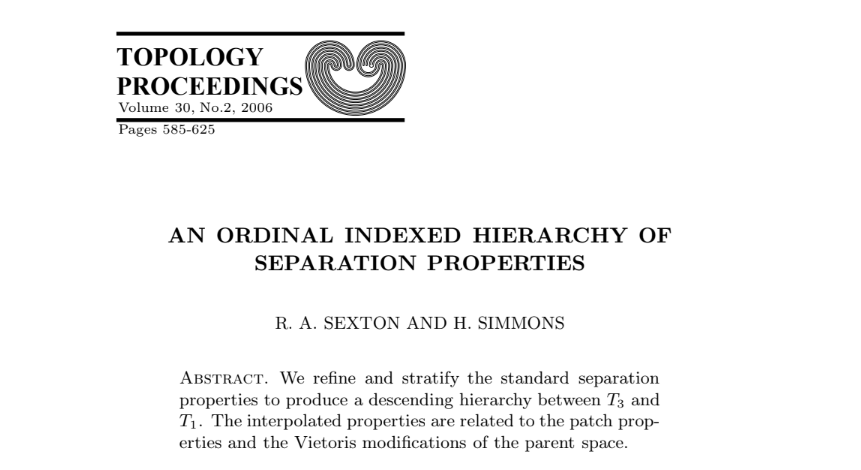
\includegraphics[width=0.6\textwidth]{Imagenes/Sexton2006.png}
    \end{center}
    \begin{center}
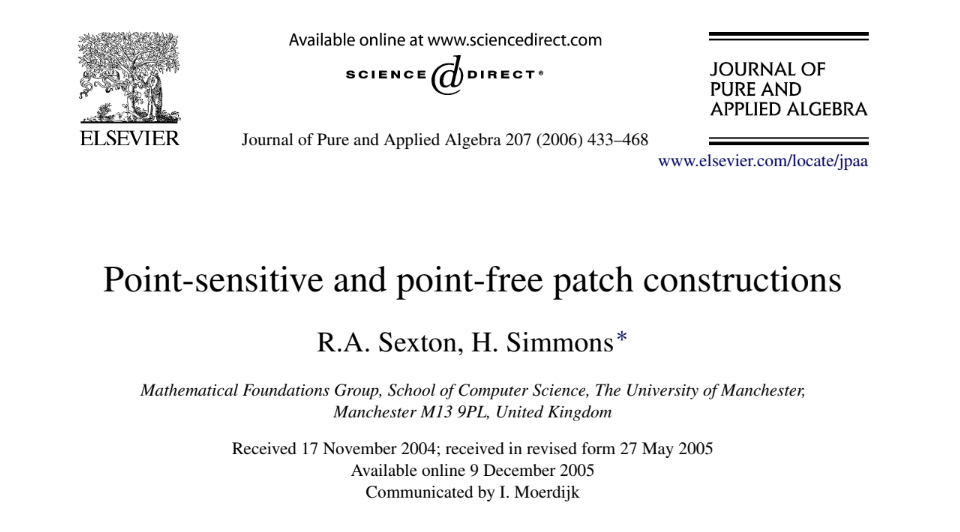
\includegraphics[width=0.6\textwidth]{Imagenes/pointsexton.png}
    \end{center}
\end{frame}

\begin{frame}{Ideas principales}
En~\cite{sexton2006ordinal,sexton2006point,sexton2003point}, Sexton y Simmons trabajan lo siguiente:
\begin{itemize}
    \item Definen los espacios \emph{empaquetados, apilados y fuertemente apilados}.
    \item Definen los marcos \emph{$\alpha$-eficientes} y \emph{$\alpha$-regulares}, donde $\alpha\in \Ord$.
    \item Introducen una jerarquia estratificada de propiedades de separación.
    \item Prueban que $\mathcal{O}S$ es eficiente si y solo si $S$ es empaquetado y apilado.
    \item Para $(G, Q)$ un par HM, relacionan las propiedades de apilamiento con los intervalos $[v_G, w_G]$.
    \item Entre otras cosas más\ldots   
\end{itemize}
\end{frame}

\begin{frame}{Marcos eficientes y espacios apilados}
    
\end{frame}

\section{Propiedades de separación inducidas por cocientes compactos}
\begin{frame}{Eficiencia y KC}

\end{frame}

\begin{frame}{Nociones de apilamiento}
    
\end{frame}

\begin{frame}{Relación con los axiomas clásicos}

\end{frame}

\begin{frame}{Interacción entre las propiedades}
    
\end{frame}

\begin{frame}{Conservatividad}
    
\end{frame}

\begin{frame}{Herencia}
    
\end{frame}

\begin{frame}{Preservación}
    
\end{frame}

\begin{frame}{Para terminar}
    
\end{frame}

\End

\begin{frame}[allowframebreaks]
\bibliographystyle{plainnat}
%\bibliographystyle{plain}
%\bibliographystyle{amsalpha}
\bibliography{research2}
\end{frame}

\begin{frame}[plain,standout]
    \centering
    \Huge{\bfseries \smiley¡Muchas gracias!\smiley}
      %In combination with \textit{plain}, \\
      %it makes a nice thank-you slide!
      \scalebox{4}{\faGithub} \par\bigskip
      \url{https://github.com/JCmonter/Apuntes/tree/main/Presentaciones} \\
      %\url{https://ctan.org/pkg/beamertheme-arguelles}
\end{frame}

\end{document}